%In this section we introduce \ourL, an action language based on \mAL that, in our opinion, is the most complete action language for epistemic planning in multi-agent domain.\\
		
The research on \mAGep\ domain, both in logic and planning, already comprehends several theoretical studies~\cite{fagin1994reasoning,moore1981reasoning,gerbrandy1999bisimulations,van2008handbook,van1997complete,van2007dynamic,baral2015action,aucher2013undecidability,bolander2015complexity,van2004dynamic} and also a variety of solvers~\cite{kominis2015beliefs,huang2017general,muise2015planning,wan2015complete,liu2018multi,le2018efp} even if, at the best of our knowledge, only~\cite{le2018efp,van2004dynamic} can reason without limitations on domains described by \lagC. 
	
%Given the complexity %(Table~\ref{table:complexity})
%that lies behind reasoning in these domains, it is clear that 
Anyway \mAGep\ solvers still have to reason on domains where the number of fluents and/or agents is limited.
This is to reduce the length of the planning problems solution that otherwise would require an  excessive quantity of resources (\ie time and memory).
For these reasons the demand of computational resources needed (for example in respect to classical planning) is one of the central problem in \mep.
	
To reduce this gap several approaches can be used:
\begin{enumerate*}[label=\roman*)]
	\item as in~\cite{kominis2015beliefs,huang2017general,muise2015planning,wan2015complete} the planning domain can be limited to a less expressive class of problems.
	
	On the other hand, when generality is required, \item heuristics can effectively reduce the resolution process, as shown in~\cite{le2018efp}.
	
	Finally another approach to follow could be \item to consider alternative representations to Kripke structures; this is what \ourL\ tries to do.
\end{enumerate*} 
	
Changing the structure is especially important because different state representation can lead to a better use of the resources, and to exploit properties of the new structure to introduce important functionalities; \eg \ourL\ could rely on the concept of \emph{bisimulation} to introduce the notion of \emph{visited states}, being bisimulation an equality criteria for \nwf\ sets.% \mep\ can be tackled from a different prospective\footnote{In the case of \ourL\ we use a set theoretical approach that introduces the epistemic planning problem to set operations.} and properties of the new structure can be exploited to introduce important functionalities; \eg \ourL\ could rely on the concept of \emph{bisimulation} to introduce the notion of \emph{visited states}, being bisimulation an equality criteria for \nwf\ sets.
	
%\ourL, as already said, is based on \mAL. The difference is in how a state is defined: in fact in \mAL\ a state is represented as Kripke structure while in \ourL\ a state is a \pos\ (for simplicity, we use the same syntax of \mAL).
%
%
%
\subsection{State} \label{subsec-contribution:state}
\FloatBarrier

	As main contribution we introduce a modified version of \mAL, called \ourL. The difference is in how a state is defined: in \mAL\ a state is represented as a Kripke structure while in \ourL\ a state is a \pos\ (\S~\ref{subsec-possibilities:possibilities}). For simplicity, we maintain the syntax used in \mAL.% where a state of the \mep\ problem is represented trough a \pos\ .
	
	The strict connection of these two structures is highlighted in~\cite{gerbrandy1999bisimulations} from the fact that a solution to a system of equations for \posS\ (Definition~\ref{def:soe_poss}) represents a decoration for a labeled graph, which is essentially a Kripke model.
	In~\cite{gerbrandy1999bisimulations}, it is also expressed that a \textquotedblleft \pos\ corresponds with a whole class of bisimilar, but structurally different, Kripke models". 
%	As is not clear what state equality in \mep\ is we leave the formal investigation of whether this structural difference is meaningful in \mep\ as future work.\\ 
	
	Let us define the usage of \posS\ as states in a \mep\ domain where the set of agents is \sAG\ and the set of fluents is \sF.
	A \pos\ %, in the sense of Definition~\ref{def:pos},
	is a function that assigns to each propositional variable $\defemph{f} \in \sF$ a truth value $\possarg{u}{\defemph{f}} \in \bra{0,1}$ and to each agent $\agent{ag} \in \sAG$ a set of \posS\ $\possarg{u}{\agent{ag}}$.
	
	A state in \mep\ has to encode the truth value of the fluents, as in classical planning, and also the beliefs of the agents about fluents and beliefs themselves.
	%In particular an agent that cannot distinguish which world is the real has.
	We defined in \S~\ref{sec:mal} how Kripke structures represent these information.
	In Figure~\ref{fig:state_as_pos} we use a \pos\ as a system of equations to encode a state (of the domain in Example~\ref{ex:coin_box}).
	
	An equation is represented in the form $\poss{u} = \bra{(\agent{ag_1}, \sigma), (\agent{ag_2}, \sigma^\prime), \dots ,\defemph{f}, \defemph{f}^\prime , \dots}$ where \agent{ag_1}, \agent{ag_2} $\in \sAG$, $\sigma, \sigma^\prime$ are sets of \posS\ and $\defemph{f}, \defemph{f}^\prime \in \sF$.
	When we write $ (\agent{ag}, \sigma)$ we mean that, in \poss{u}, the agent \agent{ag} believes that the \posS\ in $\sigma$ are plausible.
	On the other hand only if a fluent $\defemph{f}$ is present in the equation this means that the fluent itself is true in \poss{u}.
	\begin{figure}
		\centering
	%	\hspace*{-4cm}
		\subfloat[System of equations for \posS.]
		{%
			\scalebox{.8}%
			{%
				\raisebox{1.5cm}{
					$\begin{aligned}
	&\begin{cases}
		\poss{w}&= \bra{
		  	(\agent{ag},\bra{\poss{w}, \poss{w^\prime}}),
		  	(\agent{c},\bra{\poss{v}, \poss{v^\prime}}),
		  	\looking{ag},
		  	\haskey{a},
		  	\opened%
	  	}\\
		\poss{w^\prime} &=\bra{
		  	(\agent{ag},\bra{\poss{w}, \poss{w^\prime}}),
		  	(\agent{c},\bra{\poss{v}, \poss{v^\prime}}),
		  	\looking{ag},
		  	\haskey{a}, 
		  	\opened, 
		  	\head%
	 	 }\\
		\poss{v} &= \bra{
			(\agent{a},\bra{\poss{v}, \poss{v^\prime}}),
			(\agent{b},\bra{\poss{v}, \poss{v^\prime}}),
			(\agent{c},\bra{\poss{v}, \poss{v^\prime}}),
			\looking{ag},
			\haskey{a}%
		}\\
		\poss{v}^\prime &= \bra{
			(\agent{a},\bra{\poss{v}, \poss{v^\prime}}),
			(\agent{b},\bra{\poss{v}, \poss{v^\prime}}),
			(\agent{c},\bra{\poss{v}, \poss{v^\prime}}),
			\looking{ag},
			\haskey{a},
			\head%
		}\\
	\end{cases}\\
	&\text{where }\agent{ag} \in \bra{\agent{a}, \agent{b}}.
\end{aligned}$



				}%
			}%
			\label{subfig-state_as_pos:1}
		}%
		%\hspace*{.5cm}
		\subfloat[Decoration of the pointed labeled graph $(\graphG, \poss{w})$.]
		{% 
			\scalebox{0.7}%
			{%
				\raisebox{0cm}{
					

\tikzset{every picture/.style={line width=0.75pt}} %set default line width to 0.75pt        
\trimbox{0cm 0cm 0cm 1.8cm}{ 

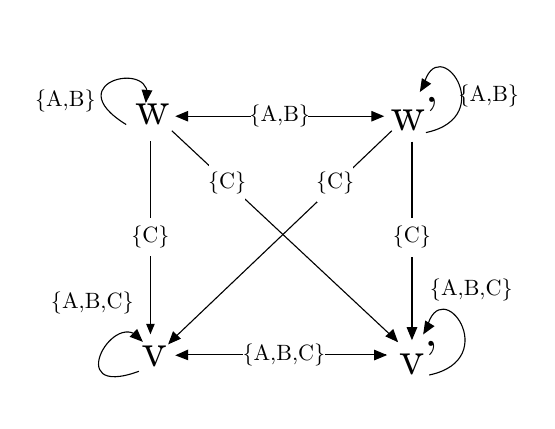
\begin{tikzpicture}[x=0.75pt,y=0.75pt,yscale=-1,xscale=1]
%uncomment if require: \path (0,237.1999969482422); %set diagram left start at 0, and has height of 237.1999969482422

%Straight Lines [id:da49380865843539024] 
\draw    (58,37.52) -- (58,129.88) ;


%Curve Lines [id:da5900505897070274] 
\draw    (55.82,18.4) .. controls (62.62,-2.4) and (11.9,8.32) .. (46.3,29.52) ;


%Shape: Triangle [id:dp7638941010979212] 
\draw  [fill={rgb, 255:red, 0; green, 0; blue, 0 }  ,fill opacity=1 ] (55.82,18.4) -- (54.11,12.94) -- (58.52,13.35) -- cycle ;
%Curve Lines [id:da33896708594278424] 
\draw    (53.81,133.72) .. controls (41.67,115.51) and (14.49,162.32) .. (52.43,148.41) ;


%Shape: Triangle [id:dp06181068467144124] 
\draw  [fill={rgb, 255:red, 0; green, 0; blue, 0 }  ,fill opacity=1 ] (53.81,133.72) -- (48.46,131.68) -- (51.51,128.48) -- cycle ;
%Straight Lines [id:da3518787636435954] 
\draw    (73.3,140.52) -- (171.3,140.52) ;


%Straight Lines [id:da9419961743422685] 
\draw    (167.3,25.52) -- (73.3,25.52) ;


%Straight Lines [id:da5282217469281014] 
\draw    (184,37.72) -- (184,130.08) ;


%Curve Lines [id:da1255493565606156] 
\draw    (191.12,127.8) .. controls (197.84,99.92) and (228.32,142.6) .. (192.32,150.2) ;


%Shape: Triangle [id:dp330887907957337] 
\draw  [fill={rgb, 255:red, 0; green, 0; blue, 0 }  ,fill opacity=1 ] (189.76,130.06) -- (190.59,124.4) -- (194.38,126.68) -- cycle ;
%Curve Lines [id:da19283464821040464] 
\draw    (189.52,11) .. controls (196.24,-16.88) and (226.72,25.8) .. (190.72,33.4) ;


%Shape: Triangle [id:dp48172892570830794] 
\draw  [fill={rgb, 255:red, 0; green, 0; blue, 0 }  ,fill opacity=1 ] (188.16,13.26) -- (188.99,7.6) -- (192.78,9.88) -- cycle ;
%Shape: Triangle [id:dp06884054633092584] 
\draw  [fill={rgb, 255:red, 0; green, 0; blue, 0 }  ,fill opacity=1 ] (184,132.72) -- (181.79,127.43) -- (186.21,127.44) -- cycle ;
%Shape: Triangle [id:dp349860096054311] 
\draw  [fill={rgb, 255:red, 0; green, 0; blue, 0 }  ,fill opacity=1 ] (171.3,140.58) -- (166.02,142.79) -- (166.02,138.37) -- cycle ;
%Shape: Triangle [id:dp5271852980265475] 
\draw  [fill={rgb, 255:red, 0; green, 0; blue, 0 }  ,fill opacity=1 ] (70.66,140.7) -- (75.94,138.31) -- (75.94,142.73) -- cycle ;
%Shape: Triangle [id:dp36308950352931935] 
\draw  [fill={rgb, 255:red, 0; green, 0; blue, 0 }  ,fill opacity=1 ] (58,129.88) -- (56.3,125.81) -- (59.7,125.81) -- cycle ;
%Shape: Triangle [id:dp1292227483684376] 
\draw  [fill={rgb, 255:red, 0; green, 0; blue, 0 }  ,fill opacity=1 ] (70.66,25.52) -- (75.94,23.31) -- (75.94,27.73) -- cycle ;
%Shape: Triangle [id:dp08607057312201727] 
\draw  [fill={rgb, 255:red, 0; green, 0; blue, 0 }  ,fill opacity=1 ] (169.94,25.52) -- (164.66,27.73) -- (164.66,23.31) -- cycle ;
%Straight Lines [id:da22782472852235425] 
\draw    (68.3,32.51) -- (176.84,133.88) ;


%Straight Lines [id:da40972295623496247] 
\draw    (174.3,32.51) -- (68.8,133.01) ;


%Shape: Triangle [id:dp9557525693039122] 
\draw  [fill={rgb, 255:red, 0; green, 0; blue, 0 }  ,fill opacity=1 ] (176.84,133.88) -- (171.64,131.49) -- (174.89,128.49) -- cycle ;
%Shape: Triangle [id:dp9360830131568407] 
\draw  [fill={rgb, 255:red, 0; green, 0; blue, 0 }  ,fill opacity=1 ] (66.99,134.94) -- (69,129.58) -- (72.22,132.61) -- cycle ;

% Text Node
\draw (59,24.32) node [scale=1.7280000000000002] [align=left] {\emphColorSlide{\poss{w}}};
% Text Node
\draw (59.8,141.22) node [scale=1.7280000000000002] [align=left] {\poss{v}};
% Text Node
\draw (17,18.32) node [scale=0.8] [align=left] {\{\agentSlide{A},\agentSlide{B}\}};
% Text Node
\draw (30,115.32) node [scale=0.8] [align=left] {\{\agentSlide{A},\agentSlide{B},\agentSlide{C}\}};
% Text Node
\draw (185.2,24.32) node [scale=1.7280000000000002] [align=left] {\poss{w'}};
% Text Node
\draw (187.11,141.72) node [scale=1.7280000000000002] [align=left] {\poss{v'}};
% Text Node
\draw (212.6,109.32) node [scale=0.8] [align=left] {\{\agentSlide{A},\agentSlide{B},\agentSlide{C}\}};
% Text Node
\draw (221,15.52) node [scale=0.8] [align=left] {\{\agentSlide{A},\agentSlide{B}\}};
% Text Node
\draw  [color={rgb, 255:red, 255; green, 255; blue, 255 }  ,draw opacity=1 ][fill={rgb, 255:red, 255; green, 255; blue, 255 }  ,fill opacity=1 ]  (106.8,16.52) -- (133.8,16.52) -- (133.8,34.52) -- (106.8,34.52) -- cycle  ;
\draw (120.3,25.52) node [scale=0.8,color={rgb, 255:red, 0; green, 0; blue, 0 }  ,opacity=1 ] [align=left] {\{\agentSlide{A},\agentSlide{B}\}};
% Text Node
\draw  [color={rgb, 255:red, 255; green, 255; blue, 255 }  ,draw opacity=1 ][fill={rgb, 255:red, 255; green, 255; blue, 255 }  ,fill opacity=1 ]  (49.5,74.7) -- (66.5,74.7) -- (66.5,92.7) -- (49.5,92.7) -- cycle  ;
\draw (58,83.7) node [scale=0.8,color={rgb, 255:red, 0; green, 0; blue, 0 }  ,opacity=1 ] [align=left] {\{\agentSlide{C}\}};
% Text Node
\draw  [color={rgb, 255:red, 255; green, 255; blue, 255 }  ,draw opacity=1 ][fill={rgb, 255:red, 255; green, 255; blue, 255 }  ,fill opacity=1 ]  (175.5,74.9) -- (192.5,74.9) -- (192.5,92.9) -- (175.5,92.9) -- cycle  ;
\draw (184,83.9) node [scale=0.8,color={rgb, 255:red, 0; green, 0; blue, 0 }  ,opacity=1 ] [align=left] {\{\agentSlide{C}\}};
% Text Node
\draw  [color={rgb, 255:red, 255; green, 255; blue, 255 }  ,draw opacity=1 ][fill={rgb, 255:red, 255; green, 255; blue, 255 }  ,fill opacity=1 ]  (86.5,48.7) -- (103.5,48.7) -- (103.5,66.7) -- (86.5,66.7) -- cycle  ;
\draw (95,57.7) node [scale=0.8,color={rgb, 255:red, 0; green, 0; blue, 0 }  ,opacity=1 ] [align=left] {\{\agentSlide{C}\}};
% Text Node
\draw  [color={rgb, 255:red, 255; green, 255; blue, 255 }  ,draw opacity=1 ][fill={rgb, 255:red, 255; green, 255; blue, 255 }  ,fill opacity=1 ]  (138.5,48.7) -- (155.5,48.7) -- (155.5,66.7) -- (138.5,66.7) -- cycle  ;
\draw (147,57.7) node [scale=0.8,color={rgb, 255:red, 0; green, 0; blue, 0 }  ,opacity=1 ] [align=left] {\{\agentSlide{C}\}};
% Text Node
\draw  [color={rgb, 255:red, 255; green, 255; blue, 255 }  ,draw opacity=1 ][fill={rgb, 255:red, 255; green, 255; blue, 255 }  ,fill opacity=1 ]  (102.8,131.52) -- (141.8,131.52) -- (141.8,149.52) -- (102.8,149.52) -- cycle  ;
\draw (122.3,140.52) node [scale=0.8,color={rgb, 255:red, 0; green, 0; blue, 0 }  ,opacity=1 ] [align=left] {\{\agentSlide{A},\agentSlide{B},\agentSlide{C}\}};


\end{tikzpicture}
}

				}%
			}%
			\label{subfig-state_as_pos:2}%
		}
		\caption{Representation of the possibility \poss{w} after the execution of the actions \distract{C}{A};\open{A} on the initial state of Example~\ref{ex:coin_box}. The \pos\ is expanded to its system of equation for clarity.}
		\label{fig:state_as_pos}
	\end{figure}%
%	

	It is clear that a \pos\ correspond to a decoration of a pointed labeled graph and therefore to a unique Kripke model up to bisimulation.
	The representation through \posS\ allows, in our opinion, a more clear and concise view of the state. That is because each state is represented by a single \pos;
	\eg Figure~\ref{fig:state_as_pos} is represented by \poss{w}= \bra{(\agent{ag},\bra{\poss{w}, \poss{w^\prime}}),(\agent{c},\bra{\poss{v}, \poss{v^\prime}}),\looking{ag},\haskey{a},\opened} where \agent{ag} $\in \bra{\agent{A}, \agent{B}}$.
%
%
%
\FloatBarrier
\subsection{State equality through Bisimulation} \label{subsec-contribution:bisim}
\FloatBarrier

	One of the reasons we chose to use \posS\ as states is to exploit this new structure to introduce new functionalities to \mep.
	In fact having the states described as \posS, which are strongly related to \nwf\ sets, help us to introduce the concept of \emph{visited states}, a core idea in planning.
	
	As said before, a \pos\ in the sense of decoration, represents all the Kripke structures bisimilar to the decoration itself.
	This means that with \posS\ we can exploit bisimulation to capture the idea of equality between states.
	In fact, given two bisimilar decorations (or labeled graphs), these, even with structural differences, are represented by the same \pos.
	On the other hand this is not true when it comes to Kripke structures.
	This idea is best described through  graphical representation; therefore we will use Figure~\ref{fig:equality} to explain this concept.
	
	As an example, let us introduce two  new actions: \flip{} and \tell{ag}{}.
	The first one is an ontic action, where an agent inverts the position of the coin; the observability of this action depends on the fluents \texttt{looking}.
	On the other hand, \tell{ag}{} means that an agent announces to \agent{ag} the position in which she thinks the coin lies while all the other agents are oblivious.
	
	Assuming that the coin lies tails up and given a sequence of action instances $\Delta = \peek{B};\distract{B}{C};\flip{C};\tell{B}{C}$\footnote{We recall that in \cite{baral2015action} an action instance is represented as $\mathtt{action}\tuple{\agent{ag}}$ where \agent{ag} is the agent that executes $\mathtt{action}$.} we show in Figure~\ref{subfig-complete:equality} the result of applying $\Delta$ in a slightly modified initial state of Example~\ref{ex:coin_box} where $\C_{\bra{A,B,C}}$(\opened\ $\wedge \neg \looking{A}$).
	In Figure~\ref{subfig-reduced:equality}, it is represented a Kripke structure that has structural differences in respect to the one in Figure~\ref{subfig-complete:equality}. This means that these two Kripke structures represent two different states in \mAL\ even if they are intuitively the same.
	On the contrary, if we think in term of \posS, both the Kripke structures of Figure~\ref{fig:equality} are represented by \pos\ \begin{center}
  \poss{r_1}=\bra{
    (\agent{a}, \bra{\poss{s_0}, \poss{s_1}}),
    (\agent{b}, \bra{\poss r_1}),
    (\agent{c}, \bra{\poss r_1}),
    \looking c,
    \haskey{a},
	\opened,
	\head}.
\end{center}

	
	\begin{figure}
		\centering
		\subfloat[The resulting Kripke structure after the execution of $\Delta$.]{\scalebox{.4}{\tikzset{every picture/.style={line width=0.75pt}} %set default line width to 0.75pt        

\trimbox{0cm 0cm 0cm 1.8cm}{ 
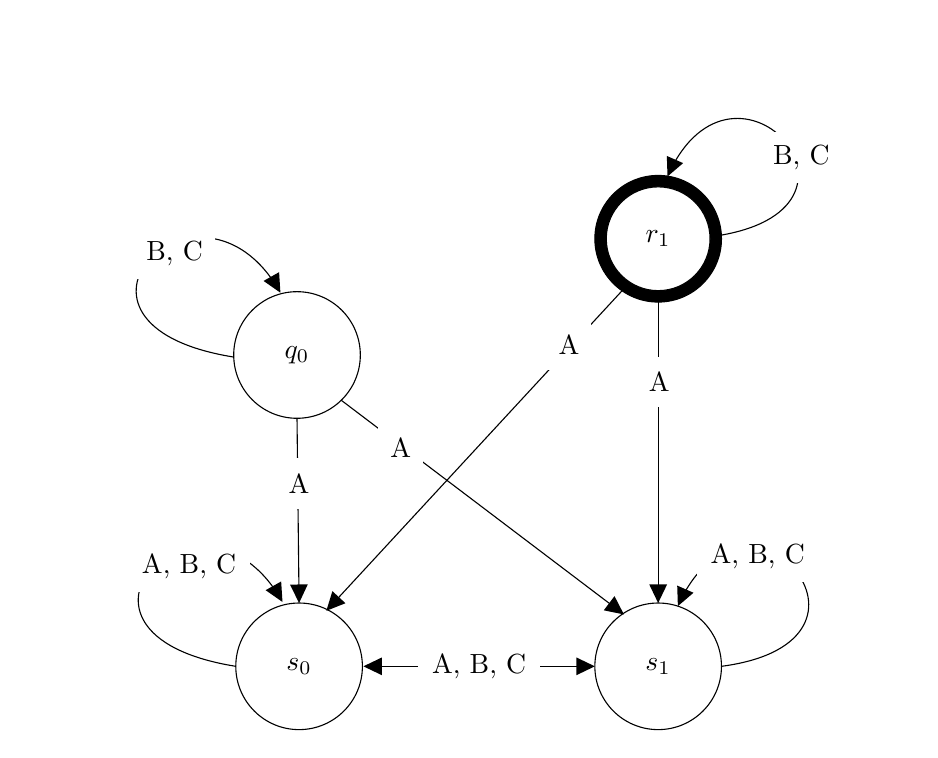
\begin{tikzpicture}[x=0.75pt,y=0.75pt,yscale=-1,xscale=1]
%uncomment if require: \path (0,369); %set diagram left start at 0, and has height of 369

%Shape: Circle [id:dp4758801382807807] 
\draw   (93.5,322) .. controls (93.5,305.16) and (107.16,291.5) .. (124,291.5) .. controls (140.84,291.5) and (154.5,305.16) .. (154.5,322) .. controls (154.5,338.84) and (140.84,352.5) .. (124,352.5) .. controls (107.16,352.5) and (93.5,338.84) .. (93.5,322) -- cycle ;
%Shape: Circle [id:dp5495909764900969] 
\draw   (266.5,322) .. controls (266.5,305.16) and (280.16,291.5) .. (297,291.5) .. controls (313.84,291.5) and (327.5,305.16) .. (327.5,322) .. controls (327.5,338.84) and (313.84,352.5) .. (297,352.5) .. controls (280.16,352.5) and (266.5,338.84) .. (266.5,322) -- cycle ;
%Straight Lines [id:da0065340714279329415] 
\draw    (157,322) -- (264.5,322) ;
\draw [shift={(266.5,322)}, rotate = 180] [fill={rgb, 255:red, 0; green, 0; blue, 0 }  ][line width=0.75]  [draw opacity=0] (8.93,-4.29) -- (0,0) -- (8.93,4.29) -- cycle    ;
\draw [shift={(155,322)}, rotate = 0] [fill={rgb, 255:red, 0; green, 0; blue, 0 }  ][line width=0.75]  [draw opacity=0] (8.93,-4.29) -- (0,0) -- (8.93,4.29) -- cycle    ;
%Curve Lines [id:da8764232980193448] 
\draw    (93.5,322) .. controls (-5.5,306.08) and (76.67,223.33) .. (115.42,289.98) ;
\draw [shift={(116,291)}, rotate = 240.66] [fill={rgb, 255:red, 0; green, 0; blue, 0 }  ][line width=0.75]  [draw opacity=0] (8.93,-4.29) -- (0,0) -- (8.93,4.29) -- cycle    ;

%Curve Lines [id:da9911776319478228] 
\draw    (327.5,322) .. controls (417.91,310.08) and (339.16,221.57) .. (306.98,291.93) ;
\draw [shift={(306.5,293)}, rotate = 293.78] [fill={rgb, 255:red, 0; green, 0; blue, 0 }  ][line width=0.75]  [draw opacity=0] (8.93,-4.29) -- (0,0) -- (8.93,4.29) -- cycle    ;

%Shape: Circle [id:dp7209538961655225] 
\draw  [fill={rgb, 255:red, 0; green, 0; blue, 0 }  ,fill opacity=1 ] (266.5,116) .. controls (266.5,99.16) and (280.16,85.5) .. (297,85.5) .. controls (313.84,85.5) and (327.5,99.16) .. (327.5,116) .. controls (327.5,132.84) and (313.84,146.5) .. (297,146.5) .. controls (280.16,146.5) and (266.5,132.84) .. (266.5,116) -- cycle ;
%Shape: Circle [id:dp27685421107424146] 
\draw   (92.5,172) .. controls (92.5,155.16) and (106.16,141.5) .. (123,141.5) .. controls (139.84,141.5) and (153.5,155.16) .. (153.5,172) .. controls (153.5,188.84) and (139.84,202.5) .. (123,202.5) .. controls (106.16,202.5) and (92.5,188.84) .. (92.5,172) -- cycle ;
%Shape: Circle [id:dp22158231372598314] 
\draw  [fill={rgb, 255:red, 255; green, 255; blue, 255 }  ,fill opacity=1 ] (272,116) .. controls (272,102.19) and (283.19,91) .. (297,91) .. controls (310.81,91) and (322,102.19) .. (322,116) .. controls (322,129.81) and (310.81,141) .. (297,141) .. controls (283.19,141) and (272,129.81) .. (272,116) -- cycle ;
%Straight Lines [id:da40013428570885556] 
\draw    (144.3,193.8) -- (278.91,295.79) ;
\draw [shift={(280.5,297)}, rotate = 217.15] [fill={rgb, 255:red, 0; green, 0; blue, 0 }  ][line width=0.75]  [draw opacity=0] (8.93,-4.29) -- (0,0) -- (8.93,4.29) -- cycle    ;

%Straight Lines [id:da31319417430186725] 
\draw    (281.5,139) -- (138.48,293.78) ;
\draw [shift={(137.13,295.25)}, rotate = 312.74] [fill={rgb, 255:red, 0; green, 0; blue, 0 }  ][line width=0.75]  [draw opacity=0] (8.93,-4.29) -- (0,0) -- (8.93,4.29) -- cycle    ;

%Straight Lines [id:da24005875384214737] 
\draw    (123,202.5) -- (123.98,289.5) ;
\draw [shift={(124,291.5)}, rotate = 269.36] [fill={rgb, 255:red, 0; green, 0; blue, 0 }  ][line width=0.75]  [draw opacity=0] (8.93,-4.29) -- (0,0) -- (8.93,4.29) -- cycle    ;

%Straight Lines [id:da7741558521862318] 
\draw    (297,146.5) -- (297,289.5) ;
\draw [shift={(297,291.5)}, rotate = 270] [fill={rgb, 255:red, 0; green, 0; blue, 0 }  ][line width=0.75]  [draw opacity=0] (8.93,-4.29) -- (0,0) -- (8.93,4.29) -- cycle    ;

%Shape: Circle [id:dp41523883310129905] 
%\draw   (133.5,78) .. controls (133.5,61.16) and (147.16,47.5) .. (164,47.5) .. controls (180.84,47.5) and (194.5,61.16) .. (194.5,78) .. controls (194.5,94.84) and (180.84,108.5) .. (164,108.5) .. controls (147.16,108.5) and (133.5,94.84) .. (133.5,78) -- cycle ;
%Curve Lines [id:da8202719280397651] 
%\draw    (194.5,78) .. controls (284.91,66.08) and (206.16,-22.43) .. (173.98,47.93) ;
%\draw [shift={(173.5,49)}, rotate = 293.78] [fill={rgb, 255:red, 0; green, 0; blue, 0 }  ][line width=0.75]  [draw opacity=0] (8.93,-4.29) -- (0,0) -- (8.93,4.29) -- cycle    ;

%Curve Lines [id:da5631597181878643] 
\draw    (322.5,115) .. controls (412.91,103.08) and (334.16,14.57) .. (301.98,84.93) ;
\draw [shift={(301.5,86)}, rotate = 293.78] [fill={rgb, 255:red, 0; green, 0; blue, 0 }  ][line width=0.75]  [draw opacity=0] (8.93,-4.29) -- (0,0) -- (8.93,4.29) -- cycle    ;

%Curve Lines [id:da7961284231370371] 
\draw    (92.5,173) .. controls (-6.5,157.08) and (75.67,74.33) .. (114.42,140.98) ;
\draw [shift={(115,142)}, rotate = 240.66] [fill={rgb, 255:red, 0; green, 0; blue, 0 }  ][line width=0.75]  [draw opacity=0] (8.93,-4.29) -- (0,0) -- (8.93,4.29) -- cycle    ;

%Straight Lines [id:da052907042750716116] 
%\draw    (177.5,105) -- (279.55,295.24) ;
%\draw [shift={(280.5,297)}, rotate = 241.79] [fill={rgb, 255:red, 0; green, 0; blue, 0 }  ][line width=0.75]  [draw opacity=0] (8.93,-4.29) -- (0,0) -- (8.93,4.29) -- cycle    ;

%Curve Lines [id:da9891597123428996] 
%\draw    (95.16,339.5) .. controls (-58.51,370.39) and (40.01,-87.28) .. (140.5,56) ;

%\draw [shift={(97.5,339)}, rotate = 167.09] [fill={rgb, 255:red, 0; green, 0; blue, 0 }  ][line width=0.75]  [draw opacity=0] (8.93,-4.29) -- (0,0) -- (8.93,4.29) -- cycle    ;

% Text Node
\draw  [color={rgb, 255:red, 255; green, 255; blue, 255 }  ,draw opacity=1 ][fill={rgb, 255:red, 255; green, 255; blue, 255 }  ,fill opacity=1 ]  (181.75,310) -- (239.75,310) -- (239.75,334) -- (181.75,334) -- cycle  ;
\draw (210.75,322) node   {\agent A, \agent B, \agent C};
% Text Node
\draw (124,322) node   {$\defemph  s_{0}$};
% Text Node
\draw (297,322) node   {$\defemph  s_{1}$};
% Text Node
\draw  [color={rgb, 255:red, 255; green, 255; blue, 255 }  ,draw opacity=1 ][fill={rgb, 255:red, 255; green, 255; blue, 255 }  ,fill opacity=1 ]  (42,262) -- (100,262) -- (100,286) -- (42,286) -- cycle  ;
\draw (71,274) node   {\agent A, \agent B, \agent C};
% Text Node
\draw  [color={rgb, 255:red, 255; green, 255; blue, 255 }  ,draw opacity=1 ][fill={rgb, 255:red, 255; green, 255; blue, 255 }  ,fill opacity=1 ]  (316,257) -- (374,257) -- (374,281) -- (316,281) -- cycle  ;
\draw (345,269) node   {\agent A, \agent B, \agent C};
% Text Node
\draw (297,116) node   {$\defemph   r_{1}$};
% Text Node
\draw (123,172) node   {$\defemph  q_{0}$};
% Text Node
%\draw (164,78) node   {$\defemph  r_{1}$};
% Text Node
%\draw  [color={rgb, 255:red, 255; green, 255; blue, 255 }  ,draw opacity=1 ][fill={rgb, 255:red, 255; green, 255; blue, 255 }  ,fill opacity=1 ]  (213,27) -- (251,27) -- (251,51) -- (213,51) -- cycle  ;
%\draw (232,39) node   {\agent B, \agent C};
% Text Node
\draw  [color={rgb, 255:red, 255; green, 255; blue, 255 }  ,draw opacity=1 ][fill={rgb, 255:red, 255; green, 255; blue, 255 }  ,fill opacity=1 ]  (243.5,155) -- (264.5,155) -- (264.5,179) -- (243.5,179) -- cycle  ;
\draw (254,167) node   {\agent A};
% Text Node
\draw  [color={rgb, 255:red, 255; green, 255; blue, 255 }  ,draw opacity=1 ][fill={rgb, 255:red, 255; green, 255; blue, 255 }  ,fill opacity=1 ]  (287,173) -- (308,173) -- (308,197) -- (287,197) -- cycle  ;
\draw (297.5,185) node   {\agent A};
% Text Node
%\draw  [color={rgb, 255:red, 255; green, 255; blue, 255 }  ,draw opacity=1 ][fill={rgb, 255:red, 255; green, 255; blue, 255 }  ,fill opacity=1 ]  (194.5,139) -- (215.5,139) -- (215.5,163) -- (194.5,163) -- cycle  ;
%\draw (205,151) node   {\agent A};
% Text Node
\draw  [color={rgb, 255:red, 255; green, 255; blue, 255 }  ,draw opacity=1 ][fill={rgb, 255:red, 255; green, 255; blue, 255 }  ,fill opacity=1 ]  (113.5,222) -- (134.5,222) -- (134.5,246) -- (113.5,246) -- cycle  ;
\draw (124,234) node   {\agent A};
% Text Node
\draw  [color={rgb, 255:red, 255; green, 255; blue, 255 }  ,draw opacity=1 ][fill={rgb, 255:red, 255; green, 255; blue, 255 }  ,fill opacity=1 ]  (162.5,205) -- (183.5,205) -- (183.5,229) -- (162.5,229) -- cycle  ;
\draw (173,217) node   {\agent A};
% Text Node
\draw  [color={rgb, 255:red, 255; green, 255; blue, 255 }  ,draw opacity=1 ][fill={rgb, 255:red, 255; green, 255; blue, 255 }  ,fill opacity=1 ]  (347,65) -- (385,65) -- (385,89) -- (347,89) -- cycle  ;
\draw (366,77) node   {\agent B, \agent C};
% Text Node
\draw  [color={rgb, 255:red, 255; green, 255; blue, 255 }  ,draw opacity=1 ][fill={rgb, 255:red, 255; green, 255; blue, 255 }  ,fill opacity=1 ]  (45,111) -- (83,111) -- (83,135) -- (45,135) -- cycle  ;
\draw (64,123) node   {\agent B, \agent C};
% Text Node
%\draw  [color={rgb, 255:red, 255; green, 255; blue, 255 }  ,draw opacity=1 ][fill={rgb, 255:red, 255; green, 255; blue, 255 }  ,fill opacity=1 ]  (46.5,48) -- (67.5,48) -- (67.5,72) -- (46.5,72) -- cycle  ;
%\draw (57,60) node   {\agent A};


\end{tikzpicture}
}}\label{subfig-complete:equality}}
		\hfill
		\subfloat[A Kripke structure bisimilar to the one in Figure~\ref{subfig-complete:equality}.]{\scalebox{0.4}{\tikzset{every picture/.style={line width=0.75pt}} %set default line width to 0.75pt        
\trimbox{0cm 0cm 0cm 1.8cm}{ 
\begin{tikzpicture}[x=0.75pt,y=0.75pt,yscale=-1,xscale=1]
%uncomment if require: \path (0,332); %set diagram left start at 0, and has height of 332

%Shape: Circle [id:dp09506861109760789] 
\draw   (67.5,279.5) .. controls (67.5,262.66) and (81.16,249) .. (98,249) .. controls (114.84,249) and (128.5,262.66) .. (128.5,279.5) .. controls (128.5,296.34) and (114.84,310) .. (98,310) .. controls (81.16,310) and (67.5,296.34) .. (67.5,279.5) -- cycle ;
%Shape: Circle [id:dp3674876277032001] 
\draw   (240.5,279.5) .. controls (240.5,262.66) and (254.16,249) .. (271,249) .. controls (287.84,249) and (301.5,262.66) .. (301.5,279.5) .. controls (301.5,296.34) and (287.84,310) .. (271,310) .. controls (254.16,310) and (240.5,296.34) .. (240.5,279.5) -- cycle ;
%Straight Lines [id:da686791560478396] 
\draw    (131,279.5) -- (238.5,279.5) ;
\draw [shift={(240.5,279.5)}, rotate = 180] [fill={rgb, 255:red, 0; green, 0; blue, 0 }  ][line width=0.75]  [draw opacity=0] (8.93,-4.29) -- (0,0) -- (8.93,4.29) -- cycle    ;
\draw [shift={(129,279.5)}, rotate = 0] [fill={rgb, 255:red, 0; green, 0; blue, 0 }  ][line width=0.75]  [draw opacity=0] (8.93,-4.29) -- (0,0) -- (8.93,4.29) -- cycle    ;
%Curve Lines [id:da3133467592132765] 
\draw    (67.5,279.5) .. controls (-31.5,263.58) and (50.67,180.83) .. (89.42,247.48) ;
\draw [shift={(90,248.5)}, rotate = 240.66] [fill={rgb, 255:red, 0; green, 0; blue, 0 }  ][line width=0.75]  [draw opacity=0] (8.93,-4.29) -- (0,0) -- (8.93,4.29) -- cycle    ;

%Curve Lines [id:da09866336174690571] 
\draw    (301.5,279.5) .. controls (391.91,267.58) and (313.16,179.07) .. (280.98,249.43) ;
\draw [shift={(280.5,250.5)}, rotate = 293.78] [fill={rgb, 255:red, 0; green, 0; blue, 0 }  ][line width=0.75]  [draw opacity=0] (8.93,-4.29) -- (0,0) -- (8.93,4.29) -- cycle    ;

%Shape: Circle [id:dp9019764791073822] 
\draw  [fill={rgb, 255:red, 0; green, 0; blue, 0 }  ,fill opacity=1 ] (240.5,73.5) .. controls (240.5,56.66) and (254.16,43) .. (271,43) .. controls (287.84,43) and (301.5,56.66) .. (301.5,73.5) .. controls (301.5,90.34) and (287.84,104) .. (271,104) .. controls (254.16,104) and (240.5,90.34) .. (240.5,73.5) -- cycle ;
%Shape: Circle [id:dp23164546006052256] 
\draw  [fill={rgb, 255:red, 255; green, 255; blue, 255 }  ,fill opacity=1 ] (246,73.5) .. controls (246,59.69) and (257.19,48.5) .. (271,48.5) .. controls (284.81,48.5) and (296,59.69) .. (296,73.5) .. controls (296,87.31) and (284.81,98.5) .. (271,98.5) .. controls (257.19,98.5) and (246,87.31) .. (246,73.5) -- cycle ;
%Straight Lines [id:da3406951202857561] 
\draw    (255.5,96.5) -- (112.48,251.28) ;
\draw [shift={(111.13,252.75)}, rotate = 312.74] [fill={rgb, 255:red, 0; green, 0; blue, 0 }  ][line width=0.75]  [draw opacity=0] (8.93,-4.29) -- (0,0) -- (8.93,4.29) -- cycle    ;

%Straight Lines [id:da5969218919849798] 
\draw    (271,104) -- (271,247) ;
\draw [shift={(271,249)}, rotate = 270] [fill={rgb, 255:red, 0; green, 0; blue, 0 }  ][line width=0.75]  [draw opacity=0] (8.93,-4.29) -- (0,0) -- (8.93,4.29) -- cycle    ;

%Curve Lines [id:da32162073734028385] 
\draw    (296.5,72.5) .. controls (386.91,60.58) and (308.16,-27.93) .. (275.98,42.43) ;
\draw [shift={(275.5,43.5)}, rotate = 293.78] [fill={rgb, 255:red, 0; green, 0; blue, 0 }  ][line width=0.75]  [draw opacity=0] (8.93,-4.29) -- (0,0) -- (8.93,4.29) -- cycle    ;


% Text Node
\draw  [color={rgb, 255:red, 255; green, 255; blue, 255 }  ,draw opacity=1 ][fill={rgb, 255:red, 255; green, 255; blue, 255 }  ,fill opacity=1 ]  (155.75,267.5) -- (213.75,267.5) -- (213.75,291.5) -- (155.75,291.5) -- cycle  ;
\draw (184.75,279.5) node   {\agent{A},\agent{B},\agent{C}};
% Text Node
\draw (98,279.5) node   {\defemph{s_{0}}};
% Text Node
\draw (271,279.5) node   {\defemph{s_{1}}};
% Text Node
\draw  [color={rgb, 255:red, 255; green, 255; blue, 255 }  ,draw opacity=1 ][fill={rgb, 255:red, 255; green, 255; blue, 255 }  ,fill opacity=1 ]  (16,219.5) -- (74,219.5) -- (74,243.5) -- (16,243.5) -- cycle  ;
\draw (45,231.5) node   {\agent{A},\agent{B},\agent{C}};
% Text Node
\draw  [color={rgb, 255:red, 255; green, 255; blue, 255 }  ,draw opacity=1 ][fill={rgb, 255:red, 255; green, 255; blue, 255 }  ,fill opacity=1 ]  (290,214.5) -- (348,214.5) -- (348,238.5) -- (290,238.5) -- cycle  ;
\draw (319,226.5) node   {\agent{A},\agent{B},\agent{C}};
% Text Node
\draw (271,73.5) node   {\defemph{r_{1}}};
% Text Node
\draw  [color={rgb, 255:red, 255; green, 255; blue, 255 }  ,draw opacity=1 ][fill={rgb, 255:red, 255; green, 255; blue, 255 }  ,fill opacity=1 ]  (217.5,112.5) -- (238.5,112.5) -- (238.5,136.5) -- (217.5,136.5) -- cycle  ;
\draw (228,124.5) node   {\agent{A}};
% Text Node
\draw  [color={rgb, 255:red, 255; green, 255; blue, 255 }  ,draw opacity=1 ][fill={rgb, 255:red, 255; green, 255; blue, 255 }  ,fill opacity=1 ]  (261,130.5) -- (282,130.5) -- (282,154.5) -- (261,154.5) -- cycle  ;
\draw (271.5,142.5) node   {\agent{A}};
% Text Node
\draw  [color={rgb, 255:red, 255; green, 255; blue, 255 }  ,draw opacity=1 ][fill={rgb, 255:red, 255; green, 255; blue, 255 }  ,fill opacity=1 ]  (321,22.5) -- (359,22.5) -- (359,46.5) -- (321,46.5) -- cycle  ;
\draw (340,34.5) node   {\agent{B},\agent{C}};


\end{tikzpicture}}}\label{subfig-reduced:equality}}
		%
		%\subfloat[Alternative Pictures of Von Neumann ordinals 2 and 3.]{\scalebox{1}{\begin{center}
  \poss{r_1}=\bra{
    (\agent{a}, \bra{\poss{s_0}, \poss{s_1}}),
    (\agent{b}, \bra{\poss r_1}),
    (\agent{c}, \bra{\poss r_1}),
    \looking c,
    \haskey{a},
	\opened,
	\head}.
\end{center}
}\label{subfig-soe:equality}}
		%
		\caption{Bisimilar Kripke Structures.}
		\label{fig:equality}
	\end{figure}
        %Even if it is not clear whether two different \posS\ may encode the same epistemic properties (we leave this problem for future works) t
        Thanks to the use
        of \posS\ we can capture bisimilar decoration while the same were considered different in \mAL\ and, therefore, check if a state has already been visited. 
%	It also interesting to notice that, since \posS\ are described in a set-based environment, operations on sets
	%, as we will see in \S~\ref{subsec-contribution:transfunc},
%	can be exploited to define the concept of update.
	Next we define the concept of entailment and finally the transition function in \ourL.
%
%
%
\FloatBarrier
\subsection{Entailment} \label{subsec-contribution:entail}
	
%	We firstly give a definition of entailment that resemble the one of \mAL\ (\S~\ref{sec:mal}); the difference lies, as said before, in the fact that \mAL\ bases its entailment on Kripke structures while \ourL\ defines its on \posS.
	%The concept of entailment also connected to the axiomatization proposed in Subsection 4.4 of~\cite{gerbrandy1999bisimulations}.
	
	We now %first of all 
	introduce the
	concept of entailment w.r.t. \posS.
	% (in the sense of Definition~\ref{def:fluent_formula}).
	
		\begin{definition}[entailment w.r.t. \posS]\label{def:poss_truth_fluent}
		Given the belief formulae
	$\varphi,\varphi_{1},\varphi_{2}$, a fluent \defemph{f}, an agent \agent{ag}, a group of agents $\alpha$, and a \pos\ \poss{u}:
		\begin{enumerate}[label= \emph{(}\roman*\emph{)}]
			\item $\poss{u} \models \defemph{f}$ if $\possarg{u}{\defemph{f}}= 1$;
		%	\item $\poss{u} \models \neg \defemph{f}$ if $\possarg{u}{\defemph{f}} = 0$;
			\item $\poss{u} \models \neg \phi$ if $\poss{u} \not \models \phi$;
			\item $\poss{u} \models \phi_1 \vee \phi_2$ if $\poss{u} \models
			\phi_1$ or $\poss{u} \models \phi_2$;
			\item $\poss{u} \models \phi_1 \wedge \phi_2$ if $\poss{u} \models
			\phi_1$ and $\poss{u} \models \phi_2$.
	%		\item $\poss{u} \models \varphi$ accordingly to \emph{Definition~\ref{def:poss_truth_fluent}} if $\varphi$ is a fluent formula;
			\item $\poss{u} \models \bB{ag}{\varphi}$ if for each $\poss{v} \in \possarg{u}{\agent{ag}}$, $\poss{v} \models \varphi$;%\footnote{The transitive closure is assured by the fact that when we reason with beliefs we guarantee that $\forall \varphi, \psi\in \lagC:
			%	M \models ( \bB{ag}{\varphi} \wedge  \bB{ag}{(\varphi \implies \psi)})
			%	\implies \bB{ag}{\psi}$ (what is called property \textbf{K} in Kripke structures).};
			\item $\poss{u} \models \neg \varphi$ if $\poss{u} \not\models \varphi$;
			\item $\poss{u} \models \varphi_1 \vee \varphi_2$ if $\poss{u} \models \varphi_1$ or $\poss{u}\models \varphi_2$;
			\item $\poss{u} \models \varphi_1 \wedge \varphi_2$ if $\poss{u} \models \varphi_1$ and $\poss{u}\models \varphi_2$;
			\item $\poss{u} \models \eAlpha{\varphi}$ if $\poss{u} \models
			\bB{ag}{\varphi}$ for all $\agent{ag} \in \alpha$;
%			\item[\emph{(}xi$^*$\emph{)}] $\poss{u} \models \eAlpha{\varphi}$ if $\bigcup_{\agent{ag} \in \alpha} \possarg{u}{\agent{ag}} \models \varphi$;
			\item $\poss{u} \models \cAlpha{\varphi}$ if
			$\poss{u} \models \eAlphaIter{k}{\varphi}$ for every
			$k\geq0$, where $\eAlphaIter{0}{\varphi} = \varphi$ and
			$\eAlphaIter{k+1}{\varphi}=\eAlpha{(\eAlphaIter{k}{\varphi})}$.
		\end{enumerate}
	\end{definition}

	%The operator \E\ can be restated through the set operation $\cup$:
%	\todo{Ask to prof} As the correctness and completeness of this transition function is not yet demonstrated we just present the description of the function with a brief comment on the intuition that lies behind it.
%
%
%
\subsection{Transition function} \label{subsec-contribution:transfunc}
	Finally we introduce the transition function for \ourL.
	%The transition function is based on the concept of corecursion as expressed in Subsection~1.2 of~\cite{gerbrandy1999bisimulations}. In fact, as we said in \S~\ref{subsec-possibilities:possibilities}, the class of all the \posS\ is the largest fixed point of the operator introduced in Page~\pageref{page:set_op}.
	In defining this transition function we made some assumptions:
	\begin{enumerate*}[label=\roman*)]
		\item we consider that the given initial state also specifies which world is the pointed one (as said in~\cite{baral2015action}), this allow us to relax the description of $\Phi$ in the case of announcements or sensing actions.

		Moreover \item we do not take into consideration the case in which an agent can have \emph{false beliefs}\footnote{An agent \agent{ag} has a false belief about $\varphi$ in state \defemph{s} if \defemph{s} $\models \varphi$ and \defemph{s} $\models \bB{ag}{\neg \varphi}$.} because is still an open question how to deal with them in \mep; we will try to address this problem in future works.
	\end{enumerate*} 
	The transition function relative to the domain \emph{D} is $\trfunc: \ai\times\Sigma \rightarrow \Sigma \cup \bra{\emptyset}$ where $\Sigma$ is the set of all the \posS.
	
	For the sake of readability, the abbreviations used in the following definition are explained at the end of it.
	\begin{definition}[transition function for \ourL]
		Let \defemph{a} $\in \ai$, and a \pos\ \poss{u} be given.
		If \defemph{a} is not executable in \poss{u} then\ $\trfunc(\defemph{a}, \poss{u}) =  \emptyset$
		otherwise if \defemph{a} is executable in \poss{u} :
		\begin{itemize}
			\item $\trfunc( \defemph{a}, \poss{u}) = \poss{v} \text{ if \defemph{a} is an ontic action instance and }$\\
			%	\begin{itemize}
			%	\item
				$\begin{cases}
					\possarg{v}{\defemph{f}} = \possarg{u}{\defemph{f}} &\text{ if } \defemph{f} \neq \res{a}\\
					\possarg{v}{\defemph{f}} = \res{a} &\text{ if } \defemph{f} = \res{a}
					%\res a &\text{ if } \defemph{f} \in \res{a}
				\end{cases}$
				\vspace*{0.1cm}
				\\and
				\vspace*{0.1cm}
				\\
				$\begin{cases}
					\possarg{v}{\agent{ag}} = \possarg{u}{\agent{ag}} &\text{ if } \agent{ag} \in \posoblivious\\
					\possarg{v}{\agent{ag}} = \bigcup_{\poss{w} \in \possarg{u}{\agent{ag}}} \trfunc( \defemph{a}, \poss{w}) &\text{ if } \agent{ag} \in \posfull			
				\end{cases}$
				\vspace*{0.3cm}
			%	\end{itemize}
			\item $\trfunc( \defemph{a}, \poss{u}) = \poss{v} \text{ if \defemph{a} sensed the fluent \defemph{f} }$\\
			%	\begin{itemize}
				%	\item
				$\begin{cases}
							%\trfunc( \defemph{a}, \poss{v}) \text{ s.t. } \poss{v} \in \possarg{u}{\agent{ag}} &\text{ if } \sensed{a}{f} \neq \possarg{u}{\defemph{f}}\\
					\emptyset &\text{ if } \sensed{a}{f} \neq \possarg{u}{\defemph{f}}\\
					\possarg{v}{\agent{ag}} = \possarg{u}{\agent{ag}} &\text{ if } \agent{ag} \in \posoblivious \text{ and } \sensed{a}{f} = \possarg{u}{\defemph{f}}\\
					\possarg{v}{\agent{ag}} = \bigcup_{\poss{w} \in \possarg{u}{\agent{ag}}} \trfunc( \defemph{a}, \poss{w}) &\text{ if }\agent{ag} \in \posfull \text{ and } \sensed{a}{f} = \possarg{u}{\defemph{f}}\\
					\possarg{v}{\agent{ag}} = \bigcup_{\poss{w} \in \possarg{u}{\agent{ag}}} (\trfunc( \defemph{a}, \poss{w}) \cup \trfunc( \neg\defemph{a}, \poss{w})) &\text{ if }\agent{ag} \in \pospartial \text{ and } \sensed{a}{f} = \possarg{u}{\defemph{f}}
				\end{cases}$
				\vspace*{0.3cm}
			%	\end{itemize}
			\item $\trfunc( \defemph{a}, \poss{u}) = \poss{v} \text{ if \defemph{a} announces the fluent formula $\phi$ }$\\
			%	\begin{itemize}
			%		\item
				$\begin{cases}
					%\trfunc( \defemph{a}, \poss{v}) \text{ s.t. } \poss{v} \in \possarg{u}{\agent{ag}} &\text{ if } \sensed{a}{f} \neq \possarg{u}{\defemph{f}}\\
					\emptyset &\text{ if } \poss{u} \not \models \phi\\
					\possarg{v}{\agent{ag}} = \possarg{u}{\agent{ag}} &\text{ if } \agent{ag} \in \posoblivious \text{ and } \poss{u} \models \phi\\
					\possarg{v}{\agent{ag}} = \bigcup_{\poss{w} \in \possarg{u}{\agent{ag}}} \trfunc( \defemph{a}, \poss{w}) &\text{ if } \agent{ag} \in \posfull \text{ and } \poss{u} \models \phi\\
					\possarg{v}{\agent{ag}} = \bigcup_{\poss{w} \in \possarg{u}{\agent{ag}}} (\trfunc( \defemph{a}, \poss{w}) \cup \trfunc( \neg\defemph{a}, \poss{w})) &\text{ if }\agent{ag} \in \pospartial \text{ and } \poss{u} \models \phi
				\end{cases}$
			%	\end{itemize}
		\end{itemize}
			
	\end{definition}
	{\footnotesize 
		where:
	\begin{itemize}
		\item \res{a} is the fluent modified by the action instance \defemph{a};
		
		\item \posfull, \pospartial, \posoblivious\ identify the fully observant, partially observant and oblivious agents respectively;
			
		\item \sensed{a}{f} represents the truth value of the fluent \defemph{f} determined by \defemph{a} = \possarg{u}{\defemph{f}};
			
		\item $\neg\defemph{a}$ describes the action that senses the opposite of \defemph{a}; namely \sensed{a}{\neg f}.
	\end{itemize}}
%
Note that sensing and announcement actions generate the empty set when the action effects do not respect the fluents truth values of the possibility where the action is executed. That is because epistemic action (\ie announcement or sensing) cannot change the state of the world but only the beliefs of the agent.

As example we present the execution of the sequence \distract{C}{A}; \open{A} on the initial state of Example~\ref{ex:coin_box} encoded by the \pos\ \poss{u} in Figure~\ref{subfig-our_tra_func:initial}.
	\begin{figure}
		\centering
		\subfloat[The initial state \poss{u}.]
		{% 
			\scalebox{0.95}%
			{%
					$\begin{cases}
 \poss u &= \bra{(\agent{ag},\bra{\poss{u}, \poss{u^\prime}}), \looking{ag}, \haskey{a}}\\
 \poss u^\prime &= \bra{(\agent{ag},\bra{\poss{u}, \poss{u^\prime}}), \looking{ag}, \haskey{a}, \head}
\end{cases}$

			}%
			\label{subfig-our_tra_func:initial}%
		}
		\subfloat[The state \poss{v} after executing \distract{C}{A}.]
		{%
			\scalebox{0.95}%
			{%
				$\begin{cases}
		\poss{v}&= \bra{
	     	(\agent{ag},\bra{\poss{v}, \poss{v^\prime}}),	\looking{a},
	     	\looking{b},
	     	\haskey{a}%
		}\\
			\poss{v}^\prime&= \bra{
	    	(\agent{ag},\bra{\poss{v}, \poss{v^\prime}}),
	    	\looking{a},
	    	\looking{b},
	    	\haskey{a},
	    	\head%
		}\\
\end{cases}$



			}%
			\label{subfig-our_tra_func:distract}%
		}
			\hfill	
		\subfloat[The state \poss{w} after executing \distract{C}{A};\open{a}.]
		{%
			\scalebox{0.95}%
			{%
			
					$\begin{cases}
	\poss{w}&= \bra{
		(\agent{a},\bra{\poss{w}, \poss{w^\prime}}),
		(\agent{b},\bra{\poss{w}, \poss{w^\prime}}),
 		(\agent{c},\bra{\poss{v}, \poss{v^\prime}}),
 		\looking{a},
 		\looking{b},
 		\haskey{a},
		\opened}\\
	\poss{w^\prime} &=\bra{
		(\agent{a},\bra{\poss{w}, \poss{w^\prime}}),
		(\agent{b},\bra{\poss{w}, \poss{w^\prime}}),
		(\agent{c},\bra{\poss{v}, \poss{v^\prime}}),
		\looking{a},
		\looking{b},
		\haskey{a},
		\opened,
		\head}
\end{cases}$


			}%
			\label{subfig-our_tra_func:open}%
		}
		\caption{Execution of \distract{C}{A};\open{A} in Example~\ref{ex:coin_box} (\agent{ag} $\in \bra{\agent{a}, \agent{b}, \agent{c}}$).}
		\label{fig:our_tra_func}
	\end{figure}%


